%Matteo Kumar - Leonard Schatt
% Fortgeschrittenes Physikalisches Praktikum

% Teilauswertung Alpha

\section{$\alpha$-Spektroskopie}

\subsection{Energiekalibrierung}
\label{subs:kali}

Zunächst wurde das Spektrum von Radium-226 mit einer 1mm-Blende in einem Abstand von ca 5mm gemessen, um eine Relation zwischen Kanalnummer 
und Energieinhalt in diesem herzustellen. Dabei wurden die Daten des Files Kali\_ra226\_b1\_603 zunächst geplottet (Abb. \ref{bild:kali}) 
und mit den Werten aus der Tabelle in Abb. \ref{bild:TabelleRa} verglichen.

\begin{figure}[h]
    \centering
    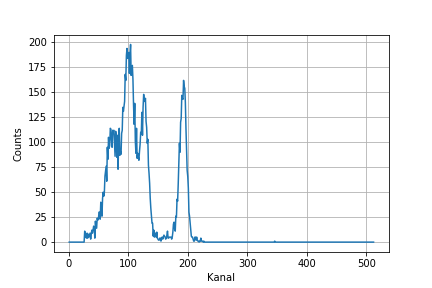
\includegraphics[scale=0.65]{Bilder/kali.png}
    \caption{Plot der Kalibrationsmessung} 
    \label{bild:kali}
\end{figure}

\begin{figure}[h]
    \centering
    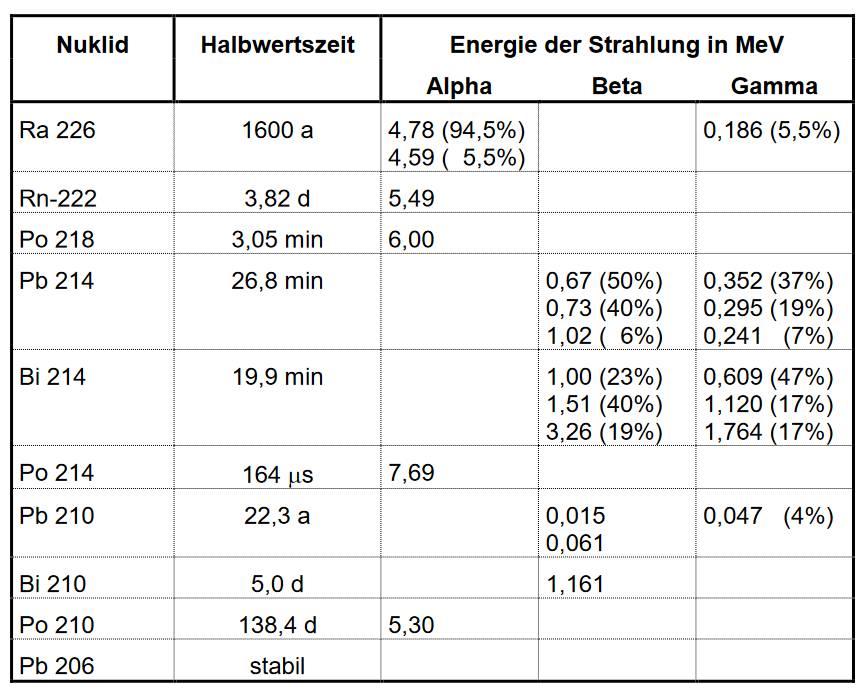
\includegraphics[scale=0.5]{Bilder/TabelleRadium.png}
    \caption{Zerfallsdaten der Ra-226-Reihe \protect \footnotemark}
    \label{bild:TabelleRa}
\end{figure}

\footnotetext{\cite{Kador2021}}

Dabei sind in der Tabelle zwei sehr kurzlebige Alphastrahler zu finden: Po-214 und Po-218. Da Po-214 die höchste Strahlenenergie hat, 
sollte der rechte einzelne Peak diesem Strahler zuzuordnen sein. Po-218 ist der rechte Peak des Dreifachpeaks zuzuordnen. Dessen 
linker Peak (Ra-226) ist für eine Kalibrierung zu schlecht aufgelöst und der mittlere aufgrund der Überlagerung zweier Strahler 
(Rn-222, Po-210) ebenfalls nicht geeignet
(\url{https://www.ld-didactic.de/software/524221en/Content/Appendix/Ra226.htm}, Stand: 14.09.21).

In den Daten wird nun der Kanal mit den maximalen Einträgen für jeden Peak gesucht. Dieser lag für Po-214 bei Kanal $193$ und 
für Po-218 bei Kanal $126$. Mit den Energie aus der Tabelle für Po-214 ($7,69$ MeV) und Po-218 ($6,00$ MeV) erhält man folgendes 
Gleichungssystem:

\begin{align*}{}
    7,69 \, MeV &= 193 \cdot m + E_0 \\
    6,00 \, MeV &= 126 \cdot m + E_0
\end{align*}

Mit der Lösung:

\begin{equation*}
    m = 0,02522388 \, MeV, \qquad E_0 = 2,82179104 \, MeV
\end{equation*}

Womit sich die Kalibrierungsgerade ergibt zu:

\begin{equation}
    E = Kanalnummer \cdot 0,02522388 \, MeV + 2,82179104 \, MeV
\end{equation}

Eine Problematik der Energiekalibrierung ist die starke Anhängigkeit der gemessenen Energien von Art und Dicke des Absorbers, wie in 
\ref{subs:abs} näher beleuchtet. Ideal wäre demnach eine Messung unter Auschluss jedweden Absorbers, also ein Vakuum.\\

\subsection{Geiger-Nutall-Regel}

Die Geiger-Nutall-Regel ist eine empirische Abschätzung zur Halbwertszeit:\\
\begin{equation}
    \lg \biggl (\frac{T_{1/2}}{1s} \biggl ) = a \cdot \frac{Z}{\sqrt{E_{\alpha}}} + b
    \label{eq:gnr}
\end{equation}


mit Konstanten a und b. Die Wertepaare für Po-214 und Po-218 aus Kapitel \ref{subs:kali} in die Formel eingesetzt liefert a und b:

\begin{equation}
    a = 1747,12602759 \sqrt{1eV} \qquad b = -56,70765593
\end{equation}

Nun kann zur Überprüfung ein Element der Zerfallsreihe von U-238 eingesetzt werden. Dies sei Rn-222; bei einer Halbwertszeit von 
$3,82$d sollte sich nach \ref{bild:TabelleRa} eine Energie von $5,49$ MeV ergeben. Es ist: \\

\begin{equation*}
    \ref{eq:gnr}  \leftrightarrow E_{\alpha} = \biggl(\,\frac{1747,12602759 \, Z}{\lg(T_{1/2})+56,70765593}\, \biggr)^2 \\
    \to E_{\alpha, Rn-222} \approx 5,56 \, MeV
\end{equation*}

Dies entspricht zwar nicht ganz dem gefordertem Wert, allerdings liegt die Abweichung nur bei ca. 1\%. Deshalb kann die 
Geiger-Nutall-Regel durchaus als bestätigt angesehen werden.

\subsection{Blendenverkleinerung}

Nun wurde eine Messung identisch zu der Kalibrationsmessung durchgeführt, mit dem einzigen Unterschied, dass anstatt der 1mm-Blende 
jetzt die 3mm-Blende verwendet wurde. Trägt man die detektierten Teilchen in den Kanäle gegen die selbigen auf, so ergibt sich der 
Graph in Abb. \ref{bild:blende}. \\

\begin{figure}[h]
    \centering
    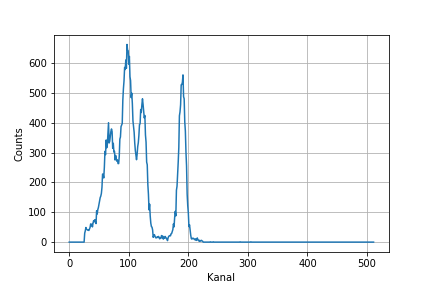
\includegraphics[scale=0.65]{Bilder/blende.png}
    \caption{Detektierte Teilchen aufgetragen gegen die Kanalnummer, 3mm-Blende}
    \label{bild:blende}
\end{figure}

Dabei fällt zunächst einmal auf, dass die Zahl der detektierten Teilchen trotz identischer Messzeit deutlich angestiegen ist. Dies ist 
allerdings zu erwarten, da eine größere Blende offensichtlich eine größere Detektorfläche freigibt. Skaliert man nun die Messung 
mit der kleineren Blende entsprechend hoch und legt diese über die Messung mit der größeren Blende, so ergibt sich Abb. 
\ref{bild:blendebeide}

\begin{figure}[h]
    \centering
    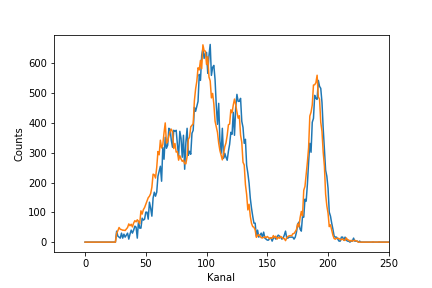
\includegraphics[scale=0.65]{Bilder/blendebeide.png}
    \caption{Vergleich der Plots für beide Blendenweiten; Werte für 1mm-Blende mit Faktor 3,35 zur Vergleichbarkeit skaliert}
    \label{bild:blendebeide}
\end{figure}

Dabei ist erkennbar, dass die Spektren beinahe identisch sind. Der Graph der größeren Blende wirkt jedoch glatter. Dies könnte 
daran liegen, dass bei kleineren Zählraten sich deren Fehler von $\sqrt{n}$ (gaußverteilt) deutlich stärker auswirkt und die Schwankungen der 
Messwerte dadurch größer ist.


\subsection{Absorption von $\alpha$-Strahlen}
\label{subs:abs}

Zur Bestimmung der Absorption von Alphastrahen wurde das Spektrum der Radiumquelle zunächst in verschiedenen Abständen zum Detektor 
aufgenommen ($1$cm, $1,5$ cm, $2$cm, $2,5$cm, $3$cm), danach in konstantem Abstand ($1 \pm 0,2$) cm, aber mit Durchgang durch 
unterschiedliche Anzahl an Schichten Mylarfolie (eine bis neun Lagen). 
Dabei betrug der Durchmesser der Blende stets $3$mm. Die Messzeit bei der Abstandsmessung wurde i.d.R. immer größer, die der 
Folienmessung betrug stets ca. $300$ s.\\

Die Graphen mit allen Abständen bzw allen und ausgewählten Lagen finden sich in den Abb. \ref{bild:abstandAlle} bis \ref{bild:lagenAusgewaehlt}. \\

\begin{figure}[h]
    \centering
    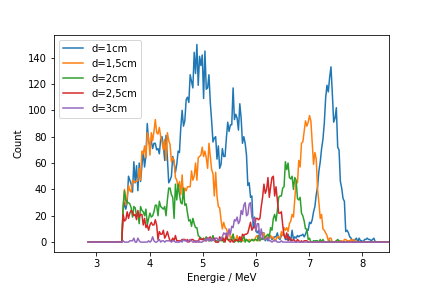
\includegraphics[scale=0.65]{Bilder/abstandAlle.png}
    \caption{Alphaspektren für verschiedene Abstände d}
    \label{bild:abstandAlle}
\end{figure}

\begin{figure}[h]
    \centering
    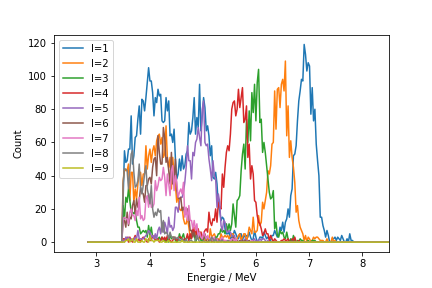
\includegraphics[scale=0.65]{Bilder/lagenAlle.png}
    \caption{Alphaspektren für alle Lagenzahlen an Mylarfolie l}
    \label{bild:lagenAlle}
\end{figure}

\begin{figure}[h]
    \centering
    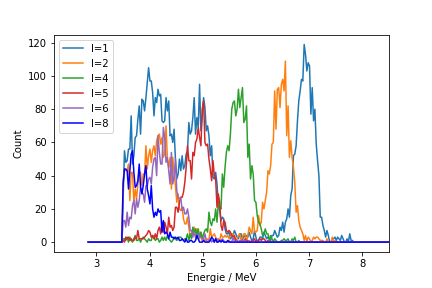
\includegraphics[scale=0.65]{Bilder/lagenAusgewaehlt.png}
    \caption{Alphaspektren für ausgewählte Lagenzahlen an Mylarfolie l}
    \label{bild:lagenAusgewaehlt}
\end{figure}

Betrachtet man die entstandenen Spektren beider Messreihen, so fallen einige Gemeinsamkeiten auf:\\
Die Anzahl der Einträge in den Kanälen, respektive die Höhe der Peaks, fallen mit zunehmenden Abstand bzw Schichtdicke, und das trotz 
teilweise längerer Messdauer. Dies ist allerdings nicht verwunderlich: Da Alphastrahen eine sehr geringe Reichweite haben, genügen schon 
kleinere Variationen in Abstand oder Dicke des Absorbermaterials, um die Transmission signifikant herabzusetzen.\\
Zudem verschiebt sich die Lage der Peaks zunehmend zu kleineren Energien hin. Das scheint auf den ersten Blick verwunderlich, sollten 
die Peaks doch den Energien der Elemente der Zerfallsreihe des Strahlers entsprechen und damit eine feste Energie haben. Jedoch 
wechselwirken die Teilchen der Alphastrahlung durch Stöße mit dem Absorbermaterial (Luft bzw Mylar) und geben so Energie ab. Dieser 
Verlust ist natürlich abhängig von der Wegstrecke durch den Absorber, was in geringeren detektierten Energien für größere Abstände 
bzw Schichtdicken führt. Diese Erklärung wird durch die Messung der Gammaspektren gestützt: Gammastrahlung ist keine Teilchenstrahlung 
sondern eine elektromagnetische Welle. Deshalb ist hier keine Verschiebung der Peaks bei Abstands- oder Absorberdickenvariation zu 
erwarten; genau dies wurde im ersten Versuchsteil bestätigt.\\
Aus der Verschiebung der Peaks ergibt sich allerdings eine praktische Konsequenz: Die Messung der Energien von Alphastrahen ist stark 
abhängig von Art und Dicke des Absorbers. Dies muss unbedigt bei der Kalibration des Messgeräts berücksichtigt werden. Da allerdings 
in der verwendeten Tabelle keine näheren Angaben gemacht wurden, gehen wir an dieser Stelle von Werten ohne Absorber aus. Die Messung 
zur Kalibration wurde mit minimalem Abstand und kleinster Blende durchgeführt, weshalb auch ein Minimum an Absorber zwischen Probe 
und Messgerät war. Deshalb ist davon auszugehen, dass die Kalibration im Wesentlichen richtig ist.\\

Trägt man nun die Quadrate der Energien (des rechten Peaks im Spektrum) gegen den Abstand (ergo Absorberdicke von Luft) bzw 
gegen die Schichtdicke der Mylarfolien (Foliendicke: $4,3 \mu$ m) auf, so ergibt sich jeweils näherugsweise eine Gerade. Dabei wurden 
bei der Mylarfolie die Messung mit den neun Lagen nicht berücksichtigt, da die Datenlage mit einer maximalen Kanalbelegung von vier zu 
gering ist. Ohnehin ist erkennbar, dass für größere Schichtzahlen die Abweichungen von der Gerade zunehmend größer werden. Mittels 
linearer Regression werden die Steigungen $m_{Luft}$ und $m_{Mylar}$ berechnet. Die Abschwächungskoeffizienten aus der 
Bethe-Bloch-Formel ergeben sich nach: \\

\begin{equation}
    k = 0,5 \cdot m \\
    \to k_{Luft} = 1,31362546 \cdot 10^{-23} \, \frac{J^2}{m}, \qquad k_{Mylar} = 1,48780223 \cdot 10^{-20} \, \frac{J^2}{m}
\end{equation}
(\cite{Jaekel1997}, S.71f) \\

Außerdem gilt: \\

\begin{equation}
    k = K \, \frac{Z \rho}{A}
\end{equation}
(\cite{Kador2021}, S. 15) \\

Damit ist: \\

\begin{equation}
    \frac{k_{Luft}}{k_{Mylar}} = \frac{Z_{Luft} \rho_{Luft} A_{Mylar}}{Z_{Mylar} \rho_{Mylar} A_{Luft}} = 
    \frac{7,22 \cdot 1,29 \cdot 10^{-3} \cdot 4,67}{2,67 \cdot 0,92 \cdot 14,44} = 0,001227
\end{equation}
 
Das Verhältnis der gemessenen Abschwächungskoeffizienten ergibt sich zu:\\

\begin{equation}
    \frac{k_{Luft}}{k_{Mylar}} = \frac{1,31362546 \cdot 10^{-23}}{1,48780223 \cdot 10^{-20}} = 0,0008829
\end{equation}

Messung und Theorie stimmen zwar in der Größenordnung überein, haben allerdings einen Fehler von ca 30\%. 

\subsection{Vermessung eines radioaktiven Zeigers}

Zuletzt wurde noch das Alphaspektrum eines alten Uhrzeigers mit radioaktiver Farbe aufgenommen. Dabei wurde aufgrund der sehr schwachen 
Strahlung die größtmögliche Blende (5mm) und ein kleinstmöglicher Abstand gewählt. Zudem betrug die Messdauer ca. einen Tag. Das 
Spektrum findet sich in Abb. \ref{bild:uhr} wieder. \\

\begin{figure}[h]
    \centering
    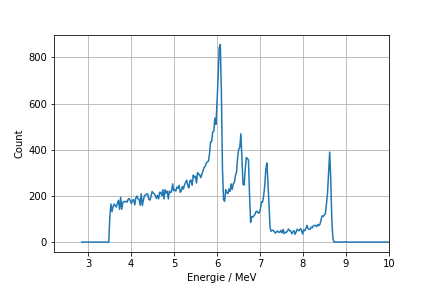
\includegraphics[scale=0.65]{Bilder/uhr.png}
    \caption{Alphaspektrum eines alten Uhrzeigers}
    \label{bild:uhr}
\end{figure}

In dem Spektrum sind die Peaks sehr scharf zu sehen. Sie liegen laut Messtabellen bei: \\

\begin{align*}
    E_0 &= 6,06 \, MeV \to Bi-212 \, (T_{1/2} = 60,5m, E = 6,05 MeV),\, Po-218 \, (T_{1/2} = 3,05m, E = 6,0 MeV) \\
    E_1 &= 6,55 \, MeV \to Rn-219 \, (T_{1/2} = 3,42s, E = 6,82 MeV), Bi-211 \, (T_{1/2} = 216s, E = 6,6 MeV)\\
    E_2 &= 6,68 \, MeV \to vgl. \, E_1 \\
    E_3 &= 7,16 \, MeV \to Po-215 \, (T_{1/2} = 1,8 \cdot 10^{-3}s, E = 7,38 MeV) \\
    E_4 &= 8,62 \, MeV \to Po-212 \, (T_{1/2} = 3 \cdot 10^{-3}s, E = 8,78 MeV) \\
\end{align*}

(\cite{Mende2016}, S. 376f)





